\pdfbookmark{Общая характеристика работы}{characteristic}             % Закладка pdf
\section*{Общая характеристика работы}

\newcommand{\actuality}{\pdfbookmark[1]{Актуальность}{actuality}\underline{\textbf{\actualityTXT}}}
\newcommand{\progress}{\pdfbookmark[1]{Разработанность темы}{progress}\underline{\textbf{\progressTXT}}}
\newcommand{\aim}{\pdfbookmark[1]{Цели}{aim}\underline{{\textbf\aimTXT}}}
\newcommand{\tasks}{\pdfbookmark[1]{Задачи}{tasks}\underline{\textbf{\tasksTXT}}}
\newcommand{\aimtasks}{\pdfbookmark[1]{Цели и задачи}{aimtasks}\aimtasksTXT}
\newcommand{\novelty}{\pdfbookmark[1]{Научная новизна}{novelty}\underline{\textbf{\noveltyTXT}}}
\newcommand{\influence}{\pdfbookmark[1]{Практическая значимость}{influence}\underline{\textbf{\influenceTXT}}}
\newcommand{\methods}{\pdfbookmark[1]{Методология и методы исследования}{methods}\underline{\textbf{\methodsTXT}}}
\newcommand{\defpositions}{\pdfbookmark[1]{Положения, выносимые на защиту}{defpositions}\underline{\textbf{\defpositionsTXT}}}
\newcommand{\reliability}{\pdfbookmark[1]{Достоверность}{reliability}\underline{\textbf{\reliabilityTXT}}}
\newcommand{\probation}{\pdfbookmark[1]{Апробация}{probation}\underline{\textbf{\probationTXT}}}
\newcommand{\contribution}{\pdfbookmark[1]{Личный вклад}{contribution}\underline{\textbf{\contributionTXT}}}
\newcommand{\publications}{\pdfbookmark[1]{Публикации}{publications}\underline{\textbf{\publicationsTXT}}}

{\actuality} 

% В настоящее время заметна тенденция цифровой трансформации, что подразумевает под собой бурное развитие информационных технологий во всех сферах деятельности человека. Основными перспективными направлениями цифровизации, на которые сделан акцент в диссертационной работе, являются цифровая трансформация транспортного комплекса и глобальная цифровизация нефтегазового сектора страны. Этот подход подразумевает не только оснащение современным технологичным оборудованием, но и глобальное изменение в подходах управления, сбора информации и средств коммуникаций. Уже сейчас основными современными информационными технологиями, встречающимися на пути трансформации являются: большие данные (Big Data), предиктивные модели на искусственных нейронных сетях (Artificial Neural Network), системы распределенного реестра (Blockchain), промышленный интернет вещей (Industrial Internet of Things, IIoT), технологии виртуальной и дополненной реальности (Virtual Reality, VR), мониторинг распределенных объектов с помощью беспилотных летательных аппаратов БПЛА (Unmanned Aerial Vehicle, UAV). В совокупности данные технологии создают необходимость в эффективной передаче больших объемов высокоскоростного трафика. Одним из путей решенияй проблемы является интенсивное развитие и внедрение беспроводных технологий.

% \fixme{В настоящее время заметна тенденция бурного развития информационных технологий во всех сферах деятельности человека. На сегодня 

% оказывает весомое влияние на нефтегазовый сектор страны. Современные компании, представляющие собой сложные многоуровневые производственные системы, для своего устойчивого развития требуют постоянного развития и совершенствования передовых технологий.  Сегодня наблюдается  бурное развитие процесса «цифровизации» нефтегазовой отрасли. Крупные международные нефтегазовые компании имеют подразделения, задачами которых является разработка и реализация принципов интеллектуального месторождения \cite{Tcharo2018} на промысле, организация безопасности на технологических объектах, развитие концепции  перехода к малолюдным системам управления добычей, транспортировкой и переработкой сырья. Уже сейчас основными современными информационными технологиями, встречающиеся в отрасли являются: большие данные (Big Data), предикстивные модели на искусственных нейронных сетях (Artificial Neural Network), системы распределенного реестра (Blockchain), промышленный интернет вещей (Industrial internet of things, IIoT), технологии виртуальной и дополненной реальности (Virtual Reality, VR), мониторинг распределенных объектов с помощью беспилотных летательных аппаратов БПЛА (Unmanned Aerial Vehicle, UAV). }
 
 
% \fixme{В совокупности данные технологии создают необходимость эффективной передачи больших объемов высокоскоростного трафика. Информационные  системы современных  сегодня содержат колоссальный объем информации высокоскоростного мультимедийного трафика. Одним из путей решения является внедрение беспроводных технологий.}

Создание современной инфраструктуры передачи данных вдоль транспортных магистралей является одной из важнейших проблем при создании нового и функционировании существующего транспортного комплекса  \cite{Vishnevsky2016_Review_of_methodology}. Одним из путей решения проблемы является интенсивное развитие и внедрение беспроводных технологий. Активное использование беспроводных сетей основывается на ряде их преимуществ по сравнению с кабельными сетями:
\begin{itemize}
    \item организация связи в труднодоступных регионах;
    \item быстрый ввод в эксплуатацию по системе подключение типа <<Подключил и Работай>> (Plug-\&-Play);
    \item сокращение капитальных затрат на создание сети; 
    \item уменьшение затрат на эксплуатацию;
    \item высокая гибкость, мобильность, масштабируемость;
    \item упрощенные требования к обслуживанию оборудования.
\end{itemize}

В рамках этого процесса возникает актуальная научно-техническая проблема повышения качества топологического проектирования беспроводной сети связи, осуществляющей мониторинг, сбор и передачу информации в центр управления с множества объектов на заданной территории.   

% В совокупности со всеми вышеизложенными перспективными направлениями беспроводные технологии являются неотъемлемой частью «цифровизации» месторождения. Отсюда возникает научно - техническая проблема организации распределенной беспроводной сети связи, соответствующая реальным требованием современного производства.

% Большой объем передачи информации  привел к еще одной из наиболее интересных тенденций цифрового развития – внедрения беспроводных технологий. Современные месторождения сегодня, помимо данных первичного сбора и обработки информации технологических параметров основных производственных объектов содержат также колоссальный объем  информации мультимедийного трафика. Сюда входят данные БПЛА по обнаружению утечек и  разрушения трубопроводов; камер видеонаблюдений; а также большой поток данных цифровых двойников, аналитики и т.д. В совокупности со всеми вышеизложенными перспективными направлениями беспроводные технологии являются неотъемлемой частью «цифровизации» месторождения.



% Процесс проектирования современной  беспроводной сети связи состоит из последовательного решения взаимосвязанных задач:

% \begin{enumerate}
%     \item обследование местности;
%     \item выбор типов технических средств и протоколов;
%     \item выбор топологической структуры сети;
%     \item анализ и оценка будущей беспроводной сети с помощью математического моделирования.
% \end{enumerate}

Диссертация посвящена актуальной проблеме синтеза топологической структуры беспроводной широкополосной сети. Задача выбора топологической структуры при проектировании является одной из важнейших задач, ошибки при которой могут привести к большим капитальным затратам и ухудшению качества обслуживания (Quality Of Service, QoS). С математической точки зрения задача синтеза топологии является сложной задачей, время счета для которой растет экспоненциально с ростом размерности. Таким образом, высокий теоретический и практический интерес к разработке новых моделей и методов оптимизации топологической структуры беспроводной широкополосной сети определяет актуальность и новизну диссертационной работы.


% Задача синтеза топологии при комплексном проектировании БШС является основной проблемой исследования в данной работе.

% В.М. Вишневский, Ю. В. Гайдамака, А.Е. Кучерявый, А.А. Ларионов, В.М. Малыш,  О.Ю. Першин, К. Е. Самуйлов, Р.Л. Смелянский и другие.

% Создание и постоянное развитие современной инфраструктуры передачи данных является одной из основных задач цифровизации. Бурное развитие беспроводных сетей во всех областях деятельности человека: интеллектуальные транспортные системы вдоль автомобильных дорог, мониторинг нефтегазовых объектов, организация современного высокоскоростного покрытия в общественных зонах обосновывают целесообразность их использования. 

% и, в частности, решающие задачу синтеза топологии В. М. Вишневский, А. А. Ларионов, В.М. Малыш, О. Ю. Першин.

{\progress} В настоящее время в России и за рубежом исследованию беспроводных сетей связи посвящен ряд работ, где рассматриваются сети для мониторинга гражданских  и промышленных объектов. Примерами таких объектов является жилые районы города, протяженные автомагистрали, линии метрополитена и железные дороги, магистральные трубопроводы и др. При исследовании проблемы синтеза топологии сети автор опирался на труды отечественных ученых, занимающихся исследованиями в области телекоммуникационных сетей: В.М. Вишневский, Ю. В. Гайдамака, Р.В. Киричек, А. Е. Кучерявый, Е. А. Кучерявый, А. А. Ларионов, В. М. Малыш,  О. Ю. Першин, К. Е. Самуйлов, Р. Л. Смелянский. Наряду с отечественными работами указанные проблемы рассматривались в работах зарубежных авторов: Е.С. Кавальканте, Х. Лиу, А.Б. Рейз, Д.Ли, Д.П. Хейман, С. Шен, Д. Бендель, У. М. Амин, Б. Брахим, Х.Э. Кызылёз и др. В работах указанных авторов рассматриваются задачи оптимального синтеза топологии сети и исследуются вопросы анализа сетей, в том числе рассматриваются оценки характеристик сетей с помощью стохастических моделей сетей массового обслуживания. 

В диссертации представлены новые математические модели задачи оптимального размещения базовых станций беспроводной широкополосной сети, предложен новый алгоритм типа ветвей и границ для решения задачи в комбинаторной форме.
Исследования доведены до разработки алгоритмов и комплексов программ, применимых для решения практических задач. Приведены результаты численных экспериментов, позволяющие оценить характеристики вычислительных методов.


{\objectresearch} являются сети специальных типов, широко представленных на практике: беспроводные широкополосные сети вдоль протяженных транспортных магистралей и беспроводные широкополосные сети с ячеистой топологией (mesh) для телекоммуникационного покрытия объектов, рассредоточенных на заданной территории.

% являются беспроводные широкополосные сети вдоль протяженных транспортных магистралей: автомобильные и железные дороги, магистральные и промысловые трубопроводы, линии метрополитена. 

% специальных типов, широко представленных на практике: БШС для контроля линейного участка и БШС с ячеистой топологией (mesh) для контроля объектов, рассредоточенных на заданной территории.

{\subjectresearch} является синтез топологической структуры беспроводной широкополосной сети.

{\aim} состоит в разработке моделей и методов оптимального размещения базовых станций для беспроводных широкополосных сетей, определяющих топологию таких сетей.

Для достижения поставленной цели были решены следующие {\tasks}:
\begin{enumerate}[beginpenalty=10000] % https://tex.stackexchange.com/a/476052/104425
  \item Проведен анализ современного состояния и перспектив развития беспроводных широкополосных сетей для обоснования  актуальности и новизны исследований в области оптимизации их топологии. 
  \item Проанализирована методика проектирования современных беспроводных широкополосных сетей с целью определения требований к решению задачи синтеза оптимальной топологии сети, а также расчета параметров беспроводной сети, необходимых для решения задач размещения базовых станций.
  \item Сформулированы математические модели для задачи оптимального размещения базовых станций беспроводной широкополосной сети с линейной топологией, разработан алгоритм типа ветвей и границ для решения указанной задачи, предложена итерационная процедура нахождения последовательности лучших решений в размещении базовых станций в рамках комплексного проектирования сети.
  \item Сформулирована математическая модель в виде задачи частично целочисленного линейного программирования для решения задач проектирования и анализа беспроводных широкополосных сетей с ячеистой топологией.
%   \item Разработан программный комплекс для расчета задачи размещения оптимального размещения базовых станций.
  \item Приведены численные эксперименты, доказывающие значимость представленных математических моделей и разработанного алгоритма.
  %   \item разработаны методы оценки характеристик производительности сети с помощью данных имитационного моделирования и методов машинного обучения. 

\end{enumerate}

 

{\novelty} результатов исследования заключается в следующем:
\begin{enumerate}[beginpenalty=10000] % https://tex.stackexchange.com/a/476052/104425

    \item Разработана новая математическая модель целочисленного линейного программирования задачи оптимального размещения базовых станций при проектировании беспроводной широкополосной сети с линейной топологией. 
    \item Разработан специальный алгоритм типа ветвей и границ для численного решения задачи в виде комбинаторной модели в экстремальной форме, учитывающей специфику размещения базовых станций беспроводной широкополосной сети для телекоммуникационного покрытия протяженных объектов. 
    % \item Разработана новая комбинаторная модель в экстремальной форме решения задачи оптимального размещения базовых станций при проектировании БШС с линейной топологией.   
    % \item Разработан специальный алгоритм типа ветвей и границ для решения численным методом сформулированной экстремальной комбинаторной задачи, учитывающий специфику размещения базовых станций БШС для телекоммуникационного покрытия протяженных объектов.
    \item Разработана новая итерационная процедура нахождения последовательности лучших решений для задачи размещения базовых станций в рамках комплексного проектирования беспроводной широкополосной сети для телекоммуникационного покрытия протяженных объектов.
    \item Разработана новая математическая модель в виде задачи частично целочисленного линейного программирования для задачи проектирования беспроводной широкополосной сети с ячеистой топологией.
    \item Разработан программный комплекс для расчета комбинаторной задачи с помощью предложенного алгоритма.

    % \item Построены новые математические модели в виде экстремальной комбинаторной задачи и задачи целочисленного линейного программирование для оптимального размещения базовых станций при проектировании БШС с линейной топологией.  
    % \item Разработан специальный алгоритм МВиГ для решения сформулированной экстремальной комбинаторной задачи размещения базовых станций вдоль линейной территории.
    % \item Разработана итерационная процедура нахождения последовательности лучших решений для задачи размещения базовых станций в рамках комплексного проектирования БШС с линейной топологией.
    % \item Разработан программный комплекс для ЭВМ расчета комбинаторной задачи.
    % \item Разработаны новые математические модели в виде задач ЦЛП для задач проектирования БШС с ячеистой топологией.
    

%   \item  \fixme{разработаны алгоритмы для анализа выполнения технологических требований и оптимального размещения базовых станций для  БШС с ячеистой топологией};
%   \item работаны имитационные модели многофазной сети массового обслуживания с зависимым временем обслуживания;
%   \item разработаны модели прогнозирования оценок характеристик производительности сети с помощью методов машинного обучения. 
\end{enumerate}

{\fieldresearch}. Диссертационная работа соответствует содержанию специальности 05.13.18 <<Математическое моделирование, численные методы и комплексы программ>>, а именно следующим пунктам специальности:
\begin{enumerate}
    \item Разработка новых математических методов моделирования объектов и явлений.
    \item Развитие качественных и приближенных аналитических методов исследования математических моделей.
    \item Реализация эффективных численных методов и алгоритмов в виде комплексов проблемно-ориентированных программ для проведения вычислительного эксперимента.
    \item Комплексные исследования научных и технических проблем с применением современной технологии математического моделирования и вычислительного эксперимента.
\end{enumerate}

{\influence}. Разработанные модели, методы и программный комплекс позволяют повысить качество проектирования беспроводных широкополосных сетей. Результаты исследования, изложенные в диссертации, получены в рамках выполнения грантов Российского фонда фундаментальных исследований \textnumero  19-07-00919,  \textnumero 19-29-06043, \textnumero 20-37-70059 и Российского научного фонда \textnumero 22-49-02023. 

% Разработанные модели, методы и программный комплекс позволяют повысить качество проектирования беспроводных широкополосных сетей. Представленные численные эксперименты в работе подтверждают эффективность при решении задачи синтеза топологии сети.
% Результаты исследования, изложенные в диссертации, получены в рамках выполнения работ при финансовой поддержке Российского фонда фундаментальных исследований по грантам \textnumero  19-07-00919,  \textnumero 19-29-06043, \textnumero 20-37-70059 и Российского научного фонда \textnumero 22-49-02023. 

% {\elaboration}. Исследования доведены до разработки алгоритмов и программ, применимых для решения практических задач. Проведены численные эксперименты, позволяющие оценить характеристики вычислительных методов.

{\methods} В работе использованы теория и методы дискретной оптимизации, математического программирования, оптимизации на конечных множествах, теории графов, методы теории вероятностей и случайных процессов, математической статистики, теории массового обслуживания. Разработка программного комплекса проводилось с использованием парадигмы объектно-ориентированного программирования.

{\defpositions}
% \begin{enumerate}[beginpenalty=10000] % https://tex.stackexchange.com/a/476052/104425
%   \item математические модели линейной задачи и алгоритм решения линейной комбинаторной задачи методом ветвей и границ;
%   \item итерационная процедура построения последовательности топологий; 
%   \item математическая модель задачи покрытия множества рассредоточенных объектов; 
%   \item имитационная модель сети массового обслуживания с зависимым распределением времени обслуживания;
%   \item регрессионные модели характеристики производительности сети, полученные с помощью методов машинного обучения.
% \end{enumerate}

\begin{enumerate}[beginpenalty=10000] % https://tex.stackexchange.com/a/476052/104425
    \item Формулировка задачи оптимального размещения базовых станций при проектировании беспроводной широкополосной сети с линейной топологией в виде целочисленного линейного программирования и в виде комбинаторной модели в экстремальной форме.
   
    % \item Математическая модель в виде задачи целочисленного линейного программирования для оптимального размещения базовых станций при проектировании беспроводной широкополосной сети с линейной топологией.
    % \item Математическая модель в виде экстремальной комбинаторной задачи для оптимального размещения базовых станций при проектировании беспроводных широкополосных сетей с линейной топологией.
    \item Специальный алгоритм типа ветвей и границ для решения сформулированной экстремальной комбинаторной задачи.
    \item Итерационная процедура нахождения последовательности лучших решений для задачи размещения базовых станций в рамках комплексного проектирования беспроводной широкополосной сети с линейной топологией.
    \item Математические модели для задач проектирования беспроводной широкополосной сети с ячеистой
    топологией.
    % \item модели прогнозирования оценок характеристик производительности сети с
    % помощью методов машинного обучения для многофазной сети массового обслуживания.
  \end{enumerate}

% В папке Documents можно ознакомиться с решением совета из Томского~ГУ (в~файле \verb+Def_positions.pdf+), где обоснованно даются рекомендации по~формулировкам защищаемых положений.

% {\reliability} \fixme{полученных результатов обеспечивается \ldots \ Результаты находятся в соответствии с результатами, полученными другими авторами.}


{\probation}
Основные положения и результаты исследования представлены и обсуждены на научных конференциях «Губкинский университет в решении вопросов нефтегазовой отрасли России» (Москва, 17-21 сентября 2018); «13-е Всероссийское совещание по проблемам управления» ВСПУ 2019 (Москва, 17-20 июня 2019); «International Conference on Distributed Computer and Communication Networks: Control, Computation, Communications» (Москва, 22-27 сентября 2019); «Губкинский университет в решении вопросов нефтегазовой отрасли России» (Москва, 24-26 сентября 2019); «Conference Management of Large-Scale System Development» (Москва, 1-3 октября 2019); «Information and Telecommunication Technologies and Mathematical Modeling of High-Tech Systems» (Москва, 13-17 апреля 2020); «Computer-aided technologies in applied mathematics» (Томск, 7-9 сентября 2020); «International Conference on Distributed Computer and Communication Networks: Control, Computation, Communications» (Москва, 14-18 сентября 2020); «Information and Telecommunication Technologies and Mathematical Modeling of High-Tech Systems» (Москва, 19-23 апреля 2021);  «5th International Scientific Conference on Information, Control, and Communication Technologies» (Астрахань, 4-7 октября 2021)


{\contribution} Основные результаты диссертации, выносимые на защиту получены автором самостоятельно.

\ifnumequal{\value{bibliosel}}{1}
{%%% Встроенная реализация с загрузкой файла через движок bibtex8. (При желании, внутри можно использовать обычные ссылки, наподобие `\cite{vakbib1,vakbib2}`).
    {\publications} Основные результаты по теме диссертации изложены в 15 печатных изданиях, 2 из которых изданы в журналах, рекомендованных ВАК, 3 — в периодических научных журналах, индексируемых Web of Science и Scopus, 10 — в сборниках трудов конференции, индексируемых РИНЦ. Зарегистрирована 1 программа для ЭВМ.
}%
{%%% Реализация пакетом biblatex через движок biber
    \begin{refsection}[bl-author, bl-registered]
        % Это refsection=1.
        % Процитированные здесь работы:
        %  * подсчитываются, для автоматического составления фразы "Основные результаты ..."
        %  * попадают в авторскую библиографию, при usefootcite==0 и стиле `\insertbiblioauthor` или `\insertbiblioauthorgrouped`
        %  * нумеруются там в зависимости от порядка команд `\printbibliography` в этом разделе.
        %  * при использовании `\insertbiblioauthorgrouped`, порядок команд `\printbibliography` в нём должен быть тем же (см. biblio/biblatex.tex)
        %
        % Невидимый библиографический список для подсчёта количества публикаций:
        \printbibliography[heading=nobibheading, section=1, env=countauthorvak,          keyword=biblioauthorvak]%
        \printbibliography[heading=nobibheading, section=1, env=countauthorwos,          keyword=biblioauthorwos]%
        \printbibliography[heading=nobibheading, section=1, env=countauthorscopus,       keyword=biblioauthorscopus]%
        \printbibliography[heading=nobibheading, section=1, env=countauthorconf,         keyword=biblioauthorconf]%
        \printbibliography[heading=nobibheading, section=1, env=countauthorother,        keyword=biblioauthorother]%
        \printbibliography[heading=nobibheading, section=1, env=countregistered,         keyword=biblioregistered]%
        \printbibliography[heading=nobibheading, section=1, env=countauthorpatent,       keyword=biblioauthorpatent]%
        \printbibliography[heading=nobibheading, section=1, env=countauthorprogram,      keyword=biblioauthorprogram]%
        \printbibliography[heading=nobibheading, section=1, env=countauthor,             keyword=biblioauthor]%
        \printbibliography[heading=nobibheading, section=1, env=countauthorvakscopuswos, filter=vakscopuswos]%
        \printbibliography[heading=nobibheading, section=1, env=countauthorscopuswos,    filter=scopuswos]%
        %
        \nocite{*}%
        %
        {\publications} Основные результаты по теме диссертации изложены в~\arabic{citeauthor}~печатных изданиях,
        \arabic{citeauthorvak} из которых изданы в журналах, рекомендованных ВАК\sloppy%
        \ifnum \value{citeauthorscopuswos}>0%
            , \arabic{citeauthorscopuswos} "--- в~периодических научных журналах, индексируемых Web of~Science и Scopus\sloppy%
        \fi%
        \ifnum \value{citeauthorconf}>0%
            , \arabic{citeauthorconf} "--- в~сборниках трудов конференции.
        \else%
            .
        \fi%
        \ifnum \value{citeregistered}=1%
            \ifnum \value{citeauthorpatent}=1%
                Зарегистрирован \arabic{citeauthorpatent} патент.
            \fi%
            \ifnum \value{citeauthorprogram}=1%
                Зарегистрирована \arabic{citeauthorprogram} программа для ЭВМ.
            \fi%
        \fi%
        \ifnum \value{citeregistered}>1%
            Зарегистрированы\ %
            \ifnum \value{citeauthorpatent}>0%
            \formbytotal{citeauthorpatent}{патент}{}{а}{}\sloppy%
            \ifnum \value{citeauthorprogram}=0 . \else \ и~\fi%
            \fi%
            \ifnum \value{citeauthorprogram}>0%
            \formbytotal{citeauthorprogram}{программ}{а}{ы}{} для ЭВМ.
            \fi%
        \fi%
        % К публикациям, в которых излагаются основные научные результаты диссертации на соискание учёной
        % степени, в рецензируемых изданиях приравниваются патенты на изобретения, патенты (свидетельства) на
        % полезную модель, патенты на промышленный образец, патенты на селекционные достижения, свидетельства
        % на программу для электронных вычислительных машин, базу данных, топологию интегральных микросхем,
        % зарегистрированные в установленном порядке.(в ред. Постановления Правительства РФ от 21.04.2016 N 335)
    \end{refsection}%
    \begin{refsection}[bl-author, bl-registered]
        % Это refsection=2.
        % Процитированные здесь работы:
        %  * попадают в авторскую библиографию, при usefootcite==0 и стиле `\insertbiblioauthorimportant`.
        %  * ни на что не влияют в противном случае
        \nocite{vakbib2}%vak
        % \nocite{patbib1}%patent
        % \nocite{progbib1}%program
        \nocite{bib1}%other
        \nocite{confbib1}%conf
    \end{refsection}%
        %
        % Всё, что вне этих двух refsection, это refsection=0,
        %  * для диссертации - это нормальные ссылки, попадающие в обычную библиографию
        %  * для автореферата:
        %     * при usefootcite==0, ссылка корректно сработает только для источника из `external.bib`. Для своих работ --- напечатает "[0]" (и даже Warning не вылезет).
        %     * при usefootcite==1, ссылка сработает нормально. В авторской библиографии будут только процитированные в refsection=0 работы.
}


% При использовании пакета \verb!biblatex! будут подсчитаны все работы, добавленные
% в файл \verb!biblio/author.bib!. Для правильного подсчёта работ в~различных
% системах цитирования требуется использовать поля:
% \begin{itemize}
%         \item \texttt{authorvak} если публикация индексирована ВАК,
%         \item \texttt{authorscopus} если публикация индексирована Scopus,
%         \item \texttt{authorwos} если публикация индексирована Web of Science,
%         \item \texttt{authorconf} для докладов конференций,
%         \item \texttt{authorpatent} для патентов,
%         \item \texttt{authorprogram} для зарегистрированных программ для ЭВМ,
%         \item \texttt{authorother} для других публикаций.
% \end{itemize}
% Для подсчёта используются счётчики:
% \begin{itemize}
%         \item \texttt{citeauthorvak} для работ, индексируемых ВАК,
%         \item \texttt{citeauthorscopus} для работ, индексируемых Scopus,
%         \item \texttt{citeauthorwos} для работ, индексируемых Web of Science,
%         \item \texttt{citeauthorvakscopuswos} для работ, индексируемых одной из трёх баз,
%         \item \texttt{citeauthorscopuswos} для работ, индексируемых Scopus или Web of~Science,
%         \item \texttt{citeauthorconf} для докладов на конференциях,
%         \item \texttt{citeauthorother} для остальных работ,
%         \item \texttt{citeauthorpatent} для патентов,
%         \item \texttt{citeauthorprogram} для зарегистрированных программ для ЭВМ,
%         \item \texttt{citeauthor} для суммарного количества работ.
% \end{itemize}
% % Счётчик \texttt{citeexternal} используется для подсчёта процитированных публикаций;
% % \texttt{citeregistered} "--- для подсчёта суммарного количества патентов и программ для ЭВМ.

% Для добавления в список публикаций автора работ, которые не были процитированы в
% автореферате, требуется их~перечислить с использованием команды \verb!\nocite! в
% \verb!Synopsis/content.tex!. % Характеристика работы по структуре во введении и в автореферате не отличается (ГОСТ Р 7.0.11, пункты 5.3.1 и 9.2.1), потому её загружаем из одного и того же внешнего файла, предварительно задав форму выделения некоторым параметрам

%Диссертационная работа была выполнена при поддержке грантов \dots

%\underline{\textbf{Объем и структура работы.}} Диссертация состоит из~введения,
%четырех глав, заключения и~приложения. Полный объем диссертации
%\textbf{ХХХ}~страниц текста с~\textbf{ХХ}~рисунками и~5~таблицами. Список
%литературы содержит \textbf{ХХX}~наименование.

\pdfbookmark{Содержание работы}{description}                          % Закладка pdf
\section*{Содержание работы}
Во \underline{\textbf{введении}} обосновывается актуальность
исследований, проводимых в~рамках данной диссертационной работы,
приводится обзор научной литературы по~изучаемой проблеме,
формулируется цель, ставятся задачи работы, излагается научная новизна
и практическая значимость представляемой работы. В~последующих главах
сначала описывается общий принцип, позволяющий \dots, а~потом идёт
апробация на частных примерах: \dots  и~\dots.


\underline{\textbf{Первая глава}} посвящена \dots

картинку можно добавить так:
\begin{figure}[ht]
    \centerfloat{
        \hfill
        \subcaptionbox{\LaTeX}{%
            
\includegraphics[scale=0.27]{latex}}
        \hfill
        \subcaptionbox{Knuth}{%
            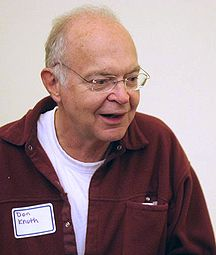
\includegraphics[width=0.25\linewidth]{knuth1}}
        \hfill
    }
    \caption{Подпись к картинке.}\label{fig:latex}
\end{figure}

Формулы в строку без номера добавляются так:
\[
    \lambda_{T_s} = K_x\frac{d{x}}{d{T_s}}, \qquad
    \lambda_{q_s} = K_x\frac{d{x}}{d{q_s}},
\]

\underline{\textbf{Вторая глава}} посвящена исследованию

\underline{\textbf{Третья глава}} посвящена исследованию

Можно сослаться на свои работы в автореферате. Для этого в файле
\verb!Synopsis/setup.tex! необходимо присвоить положительное значение
счётчику \verb!\setcounter{usefootcite}{1}!. В таком случае ссылки на
работы других авторов будут подстрочными.
Изложенные в третьей главе результаты опубликованы в~\cite{vakbib1, vakbib2}.
Использование подстрочных ссылок внутри таблиц может вызывать проблемы.

В \underline{\textbf{четвертой главе}} приведено описание

\FloatBarrier
\pdfbookmark{Заключение}{conclusion}                                  % Закладка pdf
В \underline{\textbf{заключении}} приведены основные результаты работы, которые заключаются в следующем:
%% Согласно ГОСТ Р 7.0.11-2011:
%% 5.3.3 В заключении диссертации излагают итоги выполненного исследования, рекомендации, перспективы дальнейшей разработки темы.
%% 9.2.3 В заключении автореферата диссертации излагают итоги данного исследования, рекомендации и перспективы дальнейшей разработки темы.

\begin{enumerate}
    \item Проведен анализ методики проектирования современных БШС. В рамках такой методики были исследованы проблемы синтеза топологии БШС вдоль протяженных транспортных магистралей: автомобильные дороги, трубопроводные магистрали, лини метрополитена и т.д. 
    \item Предложена новая математическая модель в виде задачи ЦЛП оптимального размещения БС с линейной топологией.
    \item Представлена новая математическая модель задачи оптимального размещения БС в комбинаторной форме. 
    % Данная модель учитывает специфику задачи для нахождения оптимального решения.
    \item Для комбинаторной модели был разработан новый специальный алгоритм типа ветвей и границ. 
    
    % Представлены результаты сравнения поиска оптимального решения с помощью МВиГ с алгоритмами решения задачи в общем виде.
    \item В рамках комплексного проектирования БШС представлена новая итерационная процедура нахождения последовательности лучших решений задачи оптимального размещения БС для случая, когда найденное оптимальное решение построение топологии сети не удовлетворяет некоторым критериями функционирования БШС, проверяемых на следующих этапах проектирования.
    \item Предложена новая математическая модель виде задачи ЧЦЛП оптимального размещения БС для покрытия множества рассредоточенных объектов. 
    \item Разработан программный комплекс для расчета задачи оптимального размещения БС  с помощью предложенного алгоритма типа ветвей и границ.
    \item Представлены результаты численных экспериментов, доказывающие эффективность предложенных моделей и методов для решения задачи синтеза топологии при проектировании БШС.
\end{enumerate}

% \begin{enumerate}
%     \item Был проведен анализ методики проектирования современных БШС. В рамках такой методики были исследованы проблемы синтеза топологии БШС вдоль протяженных участков: трубопроводные магистрали, протяженные автомобильные дороги. 
%     \item Была предложена математическая модель в виде задачи ЦЛП размещения БС с линейной топологией.
%     \item Была представлена математическая модель экстремальной задачи оптимального размещения БС в комбинаторной форме. 
%     % Данная модель учитывает специфику задачи для нахождения оптимального решения.
%     \item Для комбинаторной модели был разработан специальный алгоритм типа ветвей и границ. Представлены результаты сравнения поиска оптимального решения с помощью МВиГ с алгоритмами решения задачи в общем виде.
%     \item В рамках комплексного проектирования была представлена итерационная процедура нахождения последовательности лучших решений задачи оптимального размещения для случая, когда найденное оптимальное решение построение топологии сети не удовлетворяет некоторым критериями функционирования БШС, проверяемых на этапе моделирования процесса передачи данных.
%     \item Предложена математическая модель оптимального размещения БС для покрытия множества рассредоточенных объектов.
%     \item Разработан программный комплекс для расчета задачи оптимального размещения БС  с помощью предложенного алгоритма типа ветвей и границ.
% \end{enumerate}




% \begin{enumerate}
%   \item построены математические модели в виде экстремальной комбинаторной задачи и задачи ЦЛП для оптимального размещения базовых станций при проектировании БШС с линейной топологией;
%   \item представлен алгоритм метода ветвей и границ для задачи размещения базовых станций с линейной топологией; 
%   \item разработана итерационная процедура нахождения последовательности лучших решений для задачи размещения базовых станций в рамках комплексного проектирования БШС с линейной топологией;
%   \item разработаны математические модели для задач проектирования БШС для покрытия множества рассредоточенныз объектов;
%   \item разработаны модели прогнозирования оценок характеристик производительности сети с помощью методов машинного обучения.
% \end{enumerate}


\pdfbookmark{Литература}{bibliography}                                % Закладка pdf
При использовании пакета \verb!biblatex! список публикаций автора по теме
диссертации формируется в разделе <<\publications>>\ файла
\verb!common/characteristic.tex!  при помощи команды \verb!\nocite!

\ifdefmacro{\microtypesetup}{\microtypesetup{protrusion=false}}{} % не рекомендуется применять пакет микротипографики к автоматически генерируемому списку литературы
\urlstyle{rm}                               % ссылки URL обычным шрифтом
\ifnumequal{\value{bibliosel}}{0}{% Встроенная реализация с загрузкой файла через движок bibtex8
    \renewcommand{\bibname}{\large \bibtitleauthor}
    \nocite{*}
    \insertbiblioauthor           % Подключаем Bib-базы
    %\insertbiblioexternal   % !!! bibtex не умеет работать с несколькими библиографиями !!!
}{% Реализация пакетом biblatex через движок biber
    % Цитирования.
    %  * Порядок перечисления определяет порядок в библиографии (только внутри подраздела, если `\insertbiblioauthorgrouped`).
    %  * Если не соблюдать порядок "как для \printbibliography", нумерация в `\insertbiblioauthor` будет кривой.
    %  * Если цитировать каждый источник отдельной командой --- найти некоторые ошибки будет проще.
    %

    %% authorvak
    \nocite{IvanovVAK2019}%
    %
    %% authorwos
    \nocite{wosbib1}%
    %
    %% authorscopus
    \nocite{scbib1}%
    \nocite{Ivanov2019}%
    
    \nocite{Mukhtarov2020}%
    %
    %% authorpathent
    % \nocite{patbib1}%
    %
    %% authorprogram
    % \nocite{progbib1}%
    %
    %% authorconf
    \nocite{VishnevskyMukhtarovPershinDCCN2020_RSCI}
    \nocite{LazarevaLarionovMukhtarovITTMM2020_RSCI}
    \nocite{MukhtarovIvanovPershinDCCN2019_RSCI}
    \nocite{MukhtarovPershinVSPU2019_RSCI}
    \nocite{MukhtarovPershinMLSD2019materials_RSCI}
    \nocite{MukhtarovPershinMLSD2019works_RSCI}
    %
    %% authorother
    \nocite{VishnevskyLarionovMukhtarovICAM2020_RSCI}
    \nocite{MukhtarovPershinGUBKIN2019_RSCI}
    \nocite{MukhtarovPershinGUBKIN2018_RSCI}%

    \ifnumgreater{\value{usefootcite}}{0}{
        \begin{refcontext}[labelprefix={}]
            \ifnum \value{bibgrouped}>0
                \insertbiblioauthorgrouped    % Вывод всех работ автора, сгруппированных по источникам
            \else
                \insertbiblioauthor      % Вывод всех работ автора
            \fi
        \end{refcontext}
    }{
        \ifnum \totvalue{citeexternal}>0
            \begin{refcontext}[labelprefix=A]
                \ifnum \value{bibgrouped}>0
                    \insertbiblioauthorgrouped    % Вывод всех работ автора, сгруппированных по источникам
                \else
                    \insertbiblioauthor      % Вывод всех работ автора
                \fi
            \end{refcontext}
        \else
            \ifnum \value{bibgrouped}>0
                \insertbiblioauthorgrouped    % Вывод всех работ автора, сгруппированных по источникам
            \else
                \insertbiblioauthor      % Вывод всех работ автора
            \fi
        \fi
        %  \insertbiblioauthorimportant  % Вывод наиболее значимых работ автора (определяется в файле characteristic во второй section)
        \begin{refcontext}[labelprefix={}]
            \insertbiblioexternal            % Вывод списка литературы, на которую ссылались в тексте автореферата
        \end{refcontext}
        % Невидимый библиографический список для подсчёта количества внешних публикаций
        % Используется, чтобы убрать приставку "А" у работ автора, если в автореферате нет
        % цитирований внешних источников.
        \printbibliography[heading=nobibheading, section=0, env=countexternal, keyword=biblioexternal, resetnumbers=true]%
    }
}
\ifdefmacro{\microtypesetup}{\microtypesetup{protrusion=true}}{}
\urlstyle{tt}                               % возвращаем установки шрифта ссылок URL
